% This document is available under the Creative Commons Attribution-ShareAlike
% License; additional terms may apply. See
%   * http://creativecommons.org/licenses/by-sa/3.0/
%   * http://creativecommons.org/licenses/by-sa/3.0/legalcode
%
% Copyright 2010 Jérôme Pouiller <jezz@sysmic.org>
%

\part{Fabriquer}

{
\setbeamertemplate{background canvas}{}
\begin{frame}[plain]
  \partpage
  \begin{textblock}{10}(6,12)
    %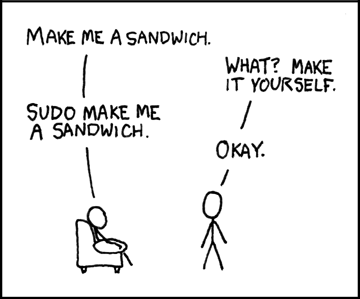
\includegraphics[height=30mm,width=30mm]{sandwich}
    \begin{quote}
      \rmfamily\textit\textbf\color{darkgray}{\large
        ``Talk is cheap. Show me the code.''}
        \vskip3mm\hspace*\fill{\small--- Torvalds, Linus (2000-08-25). Message to linux-kernel mailing list}
    \end{quote}
  \end{textblock}
\end{frame}
}

\begin{frame}
  \partpage
\end{frame}

\begin{frame}
  \tableofcontents
\end{frame}

\section{Compilation des differents éléments}

\subsection{Compilation du noyau}

\begin{frame}[fragile=singleslide]{Récupération des sources}
  Où récupérer les sources du noyau?
  \begin{enumerate}
  \item Utiliser  les sources souvent fournies.  Il arrive souvent
    qu'elles  contiennent  des  drivers particuliers  et  qu'elles
    soient déjà configurées
  \item Utiliser \cmd{git clone} (nous y reviendrons)
  \item Télecharger sur \file{kernel.org}
  \end{enumerate}
  \note[item]{Fonctionne aussi avec 2.6.37}
  \begin{lstlisting}
host$ wget http://www.kernel.org/pub/linux/kernel/v3.X/linux-3.10.32.tar.bz2
host$ tar xvjf linux-3.10.32.tar.bz2
  \end{lstlisting}
\end{frame}

\begin{frame}[fragile=singleslide]{Interface de configuration du noyau}
  \begin{itemize}
    \item Utilise Kconfig
      \begin{lstlisting}
host$ make help
host$ mkdir build
host$ make O=build ARCH=arm CROSS_COMPILE=arm-linux- menuconfig
       \end{lstlisting}
     \item  Beaucoup d'options,  mais il  y a  l'aide (\verb+<h>+)  et la
       recherche (\verb+</>+)
    \item La configuration est sauvée dans \file{.config}
    \item    \verb+at91sam9263_defconfig+   permet   de    charger   une
      configuration pré-établie pour notre carte
      \begin{lstlisting}
host$ make O=build ARCH=arm CROSS_COMPILE=arm-linux- at91sam9263_defconfig
      \end{lstlisting}
    \begin{itemize}
    \item Certains constructeur vous  fournirons un patch ajoutant une
      cible \verb+_defconfig+
    \item D'autres vous fournirons un \file{.config}
    \end{itemize}
  \end{itemize}
\end{frame}

\begin{frame}[fragile=singleslide]{Compilation du noyau}
  \begin{itemize}
  \item Vérifier les options du type de processeur
  \item Cocher NFS
  \item Le reste ne devrait pas empêcher de démarrer votre cible
  \item La compilation se lance avec
    \begin{lstlisting}
host$ make O=build ARCH=arm CROSS_COMPILE=arm-linux- XXImage
    \end{lstlisting}
  \item \verb+XX+ fait référence au format de la binaire produite:
    \begin{itemize}
    \item Le premier octet est-il du code?
    \item Respecte-t-il le format ELF?
    \item Y a-t-il un format particulier d'entête à respecter ?
    \end{itemize}
  \item Dans  le doute,  il faut consulter  la documentation  de votre
    bootloader
  \end{itemize}
\end{frame}

\begin{frame}[fragile=singleslide]{Compiler le noyau}
  Dans notre cas, nous utilisons U-Boot (standard)
  \begin{itemize}
  \item Compilation
    \begin{lstlisting}
host% apt-get install u-boot-tools
host$ make O=build ARCH=arm CROSS_COMPILE=arm-linux- uImage
    \end{lstlisting}
  \item Partage de l'image par TFTP
    \begin{lstlisting}
host% cp build/arch/arm/boot/uImage /var/lib/tftpboot/
    \end{lstlisting} % $ 
    \note[item]{C'est mieux de compiler avec -j3}
    \note[item]{Il faut les laisser démarrer en NFS}
  \end{itemize}
  \note{Parler de l'installation des modules et de l'option INSTALL\_MOD\_PATH}
\end{frame}

\begin{frame}[fragile=singleslide]{Compilation du noyau}
  Fichiers produits (ou productibles) par la compilation:
  \begin{itemize}
  \item  \verb+vmlinux+:  L'image  ELF  du  noyau.   Lisible  par  les
    debugueurs, certains flasheurs, certains bootloaders
  \item  \verb+Image+:  \verb+vmlinux+   strippé  et  préfixé  par  un
    mini-bootloader   permettant    de   sauter   sur    la   fonction
    \verb+start_kernel+ de \verb+vmlinux+.
  \item  \verb+bzImage+  et   \verb+zImage+: Comme \verb+Image+ mais compressé en \cmd{bz2} ou \cmd{gz}.
  \item  \verb+vmlinuz+: Normalement  équivalent  du \verb+bzImage+.
    %normalement, il  s'agit de\verb+vmlinux+ compressé  et strippé des
    %informations inutiles  au démarrage. Inutilisable  dans l'état, il
    %est nécessaire de lui adjoindre un bootloader pour le décompresser
    %et l'exécuter.
  \item  \verb+xipImage+  :  Idem  \verb+Image+ mais  destiné  à  être
    exécuté  directement  sur un  \emph{eeprom}  sans  être copier  en
    mémoire au préalable.
  \item  \verb+uImage+:  \verb+zImage+ avec  une  entête spéciale  pour
    \emph{u-boot}.
  \end{itemize}
%   Il est possible  de générer des image au  format SRecord en utiliant
%   \cmd{objcopy}
%   \begin{lstlisting}
% host$ objcopy -O srec vmlinux vmlinux.srec
%    \end{lstlisting}
  \note[item]{Reprendre le  slide de freeelectron très  bien foutu sur
    le sujet}
\end{frame}

\subsection{Création de l'init}

\begin{frame}[fragile=singleslide]{Démarrage du noyau}
  \begin{itemize}
  \item  A  la fin  du  démarrage  du noyau,  celui  donne  la main  à
    l'éxecutable déclaré  avec \verb+init=+. Par défaut,  il s'agit de
    \file{/sbin/init}
  \item \cmd{init} ne se termine jamais
  \item  Les  arguments  nons  utilisés  par le  noyau  sont  passé  à
    \cmd{init}
  \item On peut  estimer que notre système démarre  à partir du moment
    ou nous  obtenons un shell (c'est  en tous cas  la que la
      plupart des intégrateur Linux embarqué s'arreterons)
  \item Du moins complexe au plus complexe à démarrer:
  \begin{itemize}
    \item \verb+init=/hello-arm-static+
    \item \verb+init=/hello-arm+
    \item \verb+init=/bin/sh+
    \item \verb+init=/sbin/init+
    \end{itemize}
  \end{itemize}
  Effectuons ces tests avec le Rootfs original et un Rootfs vierge.
\end{frame}

\begin{frame}[fragile=singleslide]{Créer l'espace utilisateur}{Créer l'arborescence}
  Nous travaillerons dans un répertoire vierge
  \begin{lstlisting}
host$ mkdir nfs-root-mine
host$ cd nfs-root-mine
host$ ln -s nfs-root-mine nfs-root
  \end{lstlisting} % $
  L'arborescence classique sera:
  \vspace{-2ex}
  \begin{columns}[onlytextwidth,t]
    \begin{column}[t]{0.5\textwidth}
      \begin{itemize}
      \item bin
      \item sbin
      \item usr/bin
      \item usr/sbin
      \item etc
      \end{itemize}
    \end{column}
    \begin{column}[t]{0.5\textwidth}
      \begin{itemize}
      \item dev
      \item proc
      \item sys
      \item tmp
      \item var
      \end{itemize}
    \end{column}
  \end{columns}
  \vspace{2ex}
  Il est possible de ne pas respecter cette arborescence, mais cela
  compliquerait inutilement la chose
\end{frame}

\begin{frame}[fragile=singleslide]{Créer l'espace utilisateur}{Créer l'arborescence}
  Après le démarrage, le noyau ne trouve pas l'init:
    \begin{lstlisting}
[...]
Kernel panic - not syncing: No init found.  Try passing init= option to kernel.
    \end{lstlisting}

    Copions maintenant  \verb+hello-arm-static+ et \verb+hello-arm+ et
    essayons de démarrer avec:
    \begin{lstlisting}
[...]
Cannot open /dev/console: No such file or directory
    \end{lstlisting}
\end{frame}

\begin{frame}[fragile=singleslide]{Démarrage d'une binaire statique}
  Les fichiers devices
  \begin{itemize}
  \item Permettent de communiquer avec le noyau
  \item Il représente plus ou moins chacun un périphérique
  \item Les plus importants sont normés (\file{Documentation/devices.txt})
  \item Il est possible de les créer avec \cmd{mknod}:
    \begin{lstlisting}
host% mknod dev/console c 5 1
    \end{lstlisting}
  \item  Ce  device  est  nécessaire  pour  \cmd{printf}.   Il  serait
    possible  d'écrire un programme  ne nécessitant  aucun accès  à un
    périphérique (exemple: le service réseau echo)
  \end{itemize}
  Nous pouvons maintenant démarrer avec \verb+init=/hello-arm-static+
\end{frame}

\begin{frame}[fragile=singleslide]{Installation des bibliothèques de base}
  Les bibliothèques de base  (\cmd{libc} et apparentés) sont forcement
  fournies avec le cross-compilateur, car elles y sont intimement liés
  \begin{itemize}
  \item Liste des bibliothèques nécessaires
    \begin{lstlisting}
host$ arm-linux-ldd --root . hello-arm
    \end{lstlisting}
    \item Copie
    \begin{lstlisting}
host$ mkdir lib
host$ cp /opt/arm-linux-.../lib/ld-uClibc-1.0.9.so lib
host$ cp /opt/arm-linux-.../lib/libuClibc-1.0.9.so lib
    \end{lstlisting}
  \end{itemize}
\end{frame}

\begin{frame}[fragile=singleslide]{Installation des bibliothèques de base}
  \begin{itemize}
  \item Configuration de \cmd{ldconfig}
    \begin{lstlisting}
host$ echo /lib > etc/ld.so.conf
host$ echo /usr/lib >> etc/ld.so.conf
    \end{lstlisting}
  \item Création des liens symboliques
    \begin{lstlisting}
host$ ldconfig -r . -N
    \end{lstlisting}
  \item Création du cache. Le  cache n'est pas obligatoire, mais si il
    existe, il doit être à jour
    \note[item]{Faire un exo sur PC avec ldconfig}
    \begin{lstlisting}
host$ ldconfig -r .
    \end{lstlisting}
  \end{itemize}
  Nous pouvons maintenant démarrer avec \verb+init=/hello-arm+
\end{frame}

\subsection{Compilation de l'espace utilisateur}

\begin{frame}[fragile=singleslide]{Busybox}
  \begin{itemize}
  \item  Contient la plupart  des binaire  nécéssaire pour  démarrer un
    système
  \item Attention, ce ne  sont pas les meme outils que sur  PC. Il y a
    souvent des option non-implémentés ou des comportements différents
  \item Téléchargement
    \begin{lstlisting}
host$ wget http://busybox.net/downloads/busybox-1.23.2.tar.bz2
host$ tar xvjf busybox-1.23.2.tar.bz2
host$ mkdir build
    \end{lstlisting}
  \item On retrouve \cmd{Kconfig}
    \begin{lstlisting}
host$ make O=build CROSS_COMPILE=arm-linux- menuconfig
    \end{lstlisting}
  \end{itemize}
\end{frame}

\begin{frame}[fragile=singleslide]{Busybox}
  \begin{itemize}
  \item On trouve pleins d'outils
    \note[item]{TODO: mettre en plusieurs colonnes}
  \item    Au   minimum,    vérifions les options    \cmd{ash},   \cmd{init},    les
    \emph{Coreutils}
  \item Vérifions le chemin d'installation
    %\cmd{dmesg},   \cmd{ifconfig},   \cmd{mount},
    %\cmd{tftp}, \cmd{tar}, \cmd{reboot}, \cmd{vi}, \cmd{flashcp}
    \note[item]{TODO: mettre en plusieurs colonnes}
  %\item         Et         aussi:        \verb+CONFIG_PLATFORM_LINUX+,
  %  \verb+CONFIG_FEATURE_EDITING+,        \verb+CONFIG_FEATURE_DEVPTS+,
  %  \verb+CONFIG_LONG_OPTS+,                  \verb+CONFIG_SHOW_USAGE+,
  %  \verb+FEATURE_VERBOSE_CP_MESSAGE+, \verb+IOCTL_HEX2STR_ERROR+
  \end{itemize}
  \note[item]{TODO P2 Lister de manière exaustive}
\end{frame}

\begin{frame}[fragile=singleslide]{Installation de Busybox}
  \begin{itemize}
  \item Configurons le chemin de destination vers \file{\~/nfs}
    \begin{lstlisting}
host$ make O=build CROSS_COMPILE=arm-linux-
host$ make O=build CROSS_COMPILE=arm-linux- CONFIG_PREFIX=~/nfs install
    \end{lstlisting}
    \note[item]{Compiler avec -j3}
  \item  L'installation créé  des  liens symboliques  vers la  binaire
    \cmd{busybox}
  \item  Sans  Busybox,  toutes  ces  binaires  seraient  séparées  et
    dispersées sur une dizaine de sources
  \item Nous pouvons maintenant démarrer avec \verb+init=/bin/sh+
    \note[item] {Démarrer avec  console=ttyS0,115200 afin d'éviter les
      problème avec le jobs: Non ca ne marche pas}
  \item \verb+init=/sbin/init+ pose encore quelques problèmes.
  \end{itemize}
\end{frame}

\begin{frame}[fragile=singleslide]{Configuration de \cmd{init}}
  Il est possible de configurer \cmd{init} avec le fichier
  \file{/etc/inittab}
  \begin{itemize}
  \item Lancement automatique d'un shell
    \begin{lstlisting}
host$ echo "::askfirst:/bin/sh" > etc/inittab 
    \end{lstlisting}
  \item Appel d'un script de démarrage.
    \begin{lstlisting}
host$ echo "::sysinit:/etc/init.d/rcS" >> etc/inittab
host$ mkdir etc/init.d
host$ echo "#!/bin/sh" > etc/init.d/rcS
host$ chmod +x etc/init.d/rcS
    \end{lstlisting}
  \end{itemize}
  Documentation disponible sur la page de man \emph{inittab(5)}
  (disponible ici: \url{http://tfm.cz/man/5/inittab}).\\[2ex]
  Des  fichier de  configuration  de init  et  d'autres utilitaire  de
  busybox sont disponibles dans \file{busybox/examples}
  \note[item]{tester  avec console=ttyS0,115200  et retirer  "ttyS0 de
    l'inittab": Non ca ne marche pas}
\end{frame}

\begin{frame}[fragile=singleslide]{Compilons init}{Fichiers de configuration}
  Nous  pouvons  maintenant  démarrer avec  \cmd{init=/bin/init}  mais
  certaines fonctionnalités sont absentes (\cmd{ps}, \cmd{ifconfig}, 
  \cmd{top}, \cmd{lsusb}, etc... )\\
  Il faut monter les partitions \cmd{/proc} et \cmd{/sys}:
  \begin{lstlisting}
target% mount -t proc none /proc
target% mount -t sysfs none /sys
  \end{lstlisting}
  Automatisation du montage avec \file{inittab}:
  \begin{lstlisting}
host$ echo "::sysinit:/bin/mount -t proc none /proc" >> etc/inittab 
host$ echo "::sysinit:/bin/mount -t sysfs none /sys" >> etc/inittab 
  \end{lstlisting}
  Nos commandes semblent maintenant correctement fonctionner.
\end{frame}

\begin{frame}[fragile=singleslide]{Autres \cmd{init}}
  Il existe d'autres formes d'\cmd{init}:
  \begin{itemize}
  \item SystemV (celui que nous utilisons)
  \item runit (aussi proposé par Busybox)
  \item upstart (utilisé par Ubuntu)
  \end{itemize}
  Ces \cmd{init},  plus moderne  offre de nouvelle  fonctionnalités et
  plus de robustesse pour le système.
\end{frame}

\begin{frame}{Et si ca ne marche toujours pas?}
  \begin{itemize}
  \item Toujours commencer par  \emph{hello-static}, le moins dépendant
  \item Si il ne fonctionne  pas, recherchez dans le format de binaire
    de  la chaîne  de compilation  et avec  sa compatibilité  avec les
    options du noyaux
  \item  Si \emph{hello-static} fonctionne,  mais pas  \emph{hello} en
    dynamique, cherchez du coté des  du format de la \emph{libc} et de
    sa compatibilité avec le format de binaire \emph{hello}
  \item Si \emph{hello} fonctionne masi  que vous ne pouvez pas lancer
    de shell, cherchez du coté des devices et des droits.
  \item Si le  shell démarre mais pas init, rechechez  du coté des des
    fichiers de configuration et des devices
  \item Vérifier que votre cible  ne change pas d'IP en démarrant (ici
    dans \file{/etc/inittab})
  \item Sinon, cherchez dans les parametres passés au noyau ou dans la
    configuration
  \item Si possible, toujours tester entre chaque modification
  \end{itemize}
\end{frame}

\begin{frame}{Résumé}
  Que contient l'espace utilisateur standard?
  \begin{itemize}
  \item une arborescence
  \item des binaires
  \item des bibliothèques
  \item des fichiers devices
  \end{itemize}
\end{frame}

%\section{Quelques ajouts}
%
%\subsection{\texttt{fstab}}
%
%\begin{frame}[fragile=singleslide]{Utilisation de \file{fstab}}
%  Il  est   possible  d'automatiser  ce  montage   au  démarrage  avec
%  \file{fstab} et \cmd{mount -a}
%  \begin{lstlisting}
%host$ echo 'none /proc proc'  >> etc/fstab
%host$ echo 'none /sys  sysfs' >> etc/fstab
%target% mount -a
%  \end{lstlisting}
%
%  Nous pouvons utiliser le  fichier \file{etc/inittab} pour monter nos
%  partitions automatiquement.
%  \begin{lstlisting}
%host$ echo "::sysinit:/bin/mount -a" >> etc/inittab
%host$ echo "::shutdown:/bin/mount -r -a" >> etc/inittab
%  \end{lstlisting}
%\end{frame}
%
%\subsection{\texttt{tmpfs}}
%
%\begin{frame}[fragile=singleslide]{Filesystem temporaire}
%  Créer un  filesystem en  memoire permet de  protèger notre  flash (à
%  durée  de vie  limitée), de  garnatir que  nos système  est toujours
%  identique entre chaque démarrage et d'améliorer les performances.
%  \begin{itemize}
%    \item Création
%    \begin{lstlisting}
%host$ mkdir tmp
%    \end{lstlisting}
%  \item Ajout du \emph{stickybit} comme il se doit
%    \begin{lstlisting}
%host$ chmod +t tmp
%    \end{lstlisting}
%  \item Montage d'un filesystem contenu en mémoire
%    \begin{lstlisting}
%target% mount -t tmpfs none tmp
%host$ echo 'none /tmp tmpfs' >> etc/fstab
%    \end{lstlisting}
%  \end{itemize}
%\end{frame}
%
%\subsection{\texttt{MAKEDEV}}
%
%\begin{frame}[fragile=singleslide]{Utilisation de \cmd{MAKEDEV}}
%  \cmd{MAKEDEV} permet d'automatiser  la création des fichiers devices
%  de base
%  \begin{lstlisting}
%host$ cd dev
%host$ MAKEDEV std
%host$ MAKEDEV console
%  \end{lstlisting}
%\end{frame}
%
%\subsection{\texttt{ptmx}}
%
%\begin{frame}[fragile=singleslide]{Peudo Terminal Multiplexer}
%  \cmd{ptmx} (Peudo  Terminal Multiplexer) Permet  de facilement gérer
%  l'allocation des terminaux. (Nécessaire pour Dropbear)
%  \begin{lstlisting}
%host% mknod dev/ptmx c 5 2
%host$ mkdir dev/pts
%host$ echo 'none /dev/pts devpts' >> etc/fstab
%  \end{lstlisting}
%\end{frame}
%
%\subsection{\texttt{mdev}}
%
%\begin{frame}[fragile=singleslide]{Utilisation de \cmd{mdev}}
%  \begin{itemize}
%  \item Intégré dans Busybox
%  \item Uniquement depuis 2.6, nécessite \file{/sys} compilé et monté
%  \item Permet de créer les devices à la volée
%  \item Sur  les systèmes  très petits et  où l'utilisation  de device
%    dynamique n'est  pas nécessaire, onse passe de  \cmd{mdev} à cause
%    des dépendances avec le noyau
%  \item Création de \file{/dev} sur un disque mémoire
%    \begin{lstlisting}
%target% mount -t tmpfs none /dev
%    \end{lstlisting}
%  \item Initialisation \file{/dev} lors du démarrage
%    \begin{lstlisting}
%target% mdev -s
%    \end{lstlisting}
%  \item  Installation  de  \cmd{mdev}  comme \emph{handler}  pour  les
%    nouveaux périphériques
%    \begin{lstlisting}
%target% echo /sbin/mdev > /sys/kernel/uevent_helper
%    \end{lstlisting}
%%   \item  Automatisation du processus
%%     \begin{lstlisting}
%% host$ echo 'none /dev tmpfs' >> etc/fstab
%% host$ echo "mdev -s" >> etc/rcS
%% host$ echo "echo /sbin/mdev > /sys/kernel/uevent_helper" >> etc/rcS
%%     \end{lstlisting}
%    \note[item]{Brancher une clef USB pour faire la démonstration}
%  \end{itemize}
%\end{frame}
%
%\subsection{\texttt{resolv.conf}}
%
%\begin{frame}[fragile=singleslide]{Résolution DNS}
%  \begin{itemize}
%  \item Ajout de la résolution DNS
%    \begin{lstlisting}
%host$ echo nameserver 192.168.1.254 > etc/resolv.conf
%target% ping www.google.com
%    \end{lstlisting}
%  \item  Utiliser la  \emph{glibc}  au lieu  de  la \emph{uclibc}.  Il
%    serait    alors    nécessaire    de    configurer    le    fichier
%    \file{nsswitch.conf}.   Il  serait   possible  de   chosir  parmis
%    différente  back-ends  pour  gérer  les  authentifications  et  le
%    réseau.
%  \item  Le reste  de la  configuration réseau  s'effectue normalement
%    dans \file{/etc/network}
%  \end{itemize}
%\end{frame}
%
%\subsection{\texttt{passwd}}
%
%\begin{frame}[fragile=singleslide]{Ajouts d'utilisateurs}
%  \begin{itemize}
%  \item Ajout d'utilisateurs  (nécessaire pour beaucoup d'applications
%    dont Dropbear)
%    \begin{lstlisting}
%host$ echo 'root:x:0:0:root:/root:/bin/sh' > etc/passwd
%host$ echo 'root:x:0:' > etc/group
%host$ echo "::sysinit:login" >> etc/inittab
%    \end{lstlisting}
%  \item  \verb'root::0:0:root:/root:/bin/sh'  créerait un  utilisateur
%    sans mot de passe
%    \note[item]{TODO: Parler de shadow, mkpasswd}
%  \end{itemize}
%\end{frame}
%
%\subsection{Dropbear}
%
%\begin{frame}[fragile=singleslide]{Dropbear}
%  \begin{itemize}
%  \item Serveur et client ssh
%  \item Procédure classique (ou presque)
%    \begin{lstlisting}
%host$ wget http://matt.ucc.asn.au/dropbear/releases/dropbear-0.53.tar.bz2
%host$ tar xvjf dropbear-0.53.tar.bz2
%host$ mkdir build
%host$ ../configure --disable-zlib --host=arm-linux --build=i386 --prefix=$(pwd)/../install
%host$ make PROGRAMS="dropbear dbclient dropbearkey dropbearconvert scp"
%host$ make install
%    \end{lstlisting}
%  \end{itemize}
%\end{frame}
%
%\begin{frame}[fragile=singleslide]{Dropbear}
%  \begin{itemize}
%  \item Gestion des clef authorisées
%    \begin{lstlisting}
%host$ mkdir -p etc/dropbear
%host$ mkdir -p root/.ssh
%host$ cp ~/.ssh/authorized_keys root/.ssh
%    \end{lstlisting}%$
%  \item Génération des clef host:
%    \begin{lstlisting}
%target% dropbearkey -t rsa -f /etc/dropbear/dropbear_rsa_host_key
%target% dropbearkey -t dss -f /etc/dropbear/dropbear_dss_host_key
%target% dropbear -E
%host$ echo "ttyS0::respawn:/sbin/dropbear -E" >> etc/inittab
%host$ ssh root@target
%    \end{lstlisting}
%  \end{itemize}
%  Dropbear  nécessite un  certain  nombre de  fonctionnalité de  notre
%  Linux.  Le faire  fonctionner est  un bon  test de  compatibilité de
%  notre système
%\end{frame}
%
%\section{Bootstrapper la toolchain}
%
%\begin{frame}[fragile=singleslide]{Compiler le cross-compiler et la libc}
%  \begin{itemize}
%  \item Le compilateur et la \cmd{libc} se compile ensemble
%  \item On peut identifier la toolchain à son triplet:
%    \begin{itemize}
%    \item \verb+<CPU>-<VENDOR>-<SYSTEM>+
%    \item \verb+<SYSTEM> ~ <KERNEL>-<OS>+
%    \item \verb+<KERNEL> =+ linux
%    \item \verb+<OS>+  est une notion  plus floue: gnu,  ulibc, glibc,
%      ulibcgnueabi...
%    \end{itemize}
%  \item  Pour \cmd{gcc},  on abbrège  souvent le  triplet  en omettant
%    \verb+<VENDOR>+
%  \item Exemples:
%    \begin{itemize}
%    \item ppc85-e8541-linux-gnu % A verfieir
%    \item arm9-atmel-linux-ulibceabi % A verifier
%    \item sh4-st-unknown: Pas de libc, permet de compiler le noyau
%      et u-boot, mais pas d'application user
%    \item i586-pc-mingw32msvc: Target windows
%    \end{itemize}
%  \item Attention, ca n'est pas une science exacte
%  \end{itemize}
%\end{frame}
%
%\begin{frame}[fragile=singleslide]{Compiler le cross-compiler et la libc}
%  \begin{itemize}
%  \item 3 étapes:
%    \begin{itemize}
%    \item On compile \cmd{arm-unknown-gcc}
%    \item On configure le noyau pour installer les \emph{headers}
%    \item On  compile la  \cmd{libc} avec \cmd{arm-unknown-gcc}  et le
%      noyau préconfiguré, on compile le noyau
%    \item On compile \cmd{arm-linux-libc-gcc}
%    \end{itemize}
%  \item Difficultés :
%    \begin{itemize}
%    \item Assez complexe
%    \item Souvent des problèmes de compatibilité entre les versions
%    \end{itemize}
%  \end{itemize}
%\end{frame}
%
%\begin{frame}[fragile=singleslide]{Compiler le cross-compiler et la libc}
%  Différentes \cmd{libc}:
%  \begin{itemize}
%  \item glibc (``GNU C Library'', la vénérable)
%  \item  eglibc  (``Embedded GNU  C  Library'',  meilleur support  des
%    diverses  architectures.  Utilisée  depuis récement  sur  diverses
%    distributions ``desktop'')
%  \item newlib (utilisée par Cygwin)
%  \item µclibc (très utilisée dans l'embarqué)
%  \item  dietlibc  (encore  plus   petite  que  µlibc  destinée  à  la
%    compilation statique)
%  \item bionic (Android)
%  \end{itemize}
%\end{frame}
%
%\begin{frame}[fragile=singleslide]{Compiler la toolchain}{Crosstool-NG}
%  Crosstool-NG :
%  \begin{itemize}
%  \item Système automatisant toute la procédure et intégrant les patch
%    connu pour rendre compatible certains systèmes
%  \item Principalement maintenu par Yann Morin (cocoricco)
%  \item Il n'existe  pas de paquet, nous devons  donc le compiler nous
%    même:
%    \begin{lstlisting}
%host% apt-get install automake libtool texinfo flex bison gawk ...
%host$ wget http://crosstool-ng.org/download/crosstool-ng/crosstool-ng-1.13.4.tar.bz2
%host$ tar xvzf crosstool-ng-1.13.4.tar.bz2
%host$ cd crosstool-ng-1.13.4
%host$ ./configure && make
%host% make install
%    \end{lstlisting}
%  \end{itemize}
%\end{frame}
%
%\begin{frame}[fragile=singleslide]{Compiler la toolchain}{Crosstool-NG}
%  \begin{itemize}
%  \item Préparation du répertoire de build
%    \begin{lstlisting}
%$ mkdir ct-build ct-dl
%$ cd ct-build
%$ ct-ng help
%    \end{lstlisting}
%  \item Partons de l'exemple le plus proche de notre configuration
%    \begin{lstlisting}
%$ ct-ng list-samples
%$ ct-ng arm-unknown-linux-uclibcgnueabi
%    \end{lstlisting}
%  \item Vérifions que le l'exemple compile
%    \begin{lstlisting}
%$ ct-ng build
%    \end{lstlisting}
%  \end{itemize}
%\end{frame}
%
%\begin{frame}[fragile=singleslide]{Compiler la toolchain}{Crosstool-NG}
%  \begin{itemize}
%  \item Configurons notre chaine de compilation finale
%    \begin{lstlisting}
%$ ct-ng clean
%$ ct-ng menuconfig
%       \end{lstlisting}
%     \item Dans la configuration
%       \begin{lstlisting}
%... Prefix directory: /opt/${CT_TARGET}
%... Remove documentation
%... Build Static Toolchain
%# Documentation du CPU + man gcc + wikipedia (http://en.wikipedia.org/wiki/ARM_architecture)
%... Architecture level: armv5te
%# Page de man de gcc + documentation du CPU :
%... Emit assembly for CPU: arm926ej-s
%... Tuple's vendor string : sysmic
%... Threading implementation to use: (nptl)
%... Add support for locales
%       \end{lstlisting}
%  \end{itemize}
%\end{frame}
%
%\begin{frame}[fragile=singleslide]{Compiler la toolchain}{Crosstool-NG}
%  \begin{itemize}
%     \item Compilons
%       \begin{lstlisting}
%$ chmod 777 /opt
%$ ct-ng build
%$ ct-ng tarball
%       \end{lstlisting}
%     \item Testons en statique
%       \begin{lstlisting}[basicstyle=\ttfamily\scriptsize\color{colBasic}]
%host$ /opt/arm-sysmic-linux-uclibcgnueabi/bin/arm-sysmic-linux-uclibcgnueabi-gcc -static -Wall hello.c -o hello-mygcc-static
%target$ ./hello-mygcc-static
%       \end{lstlisting}
%     \item Testons en dynamique
%       \begin{lstlisting}[basicstyle=\ttfamily\scriptsize\color{colBasic}]
%host$ /opt/arm-sysmic-linux-uclibcgnueabi/bin/arm-sysmic-linux-uclibcgnueabi-gcc -Wall hello.c -o hello-mygcc
%target$ ./hello-mygcc
%	\end{lstlisting}
%  \end{itemize}
%\end{frame}
%
%\begin{frame}[fragile=singleslide]{Compiler la toolchain}{Crosstool-NG}
%  \begin{itemize}
%      \item Il  possible (probable) que les bibliothèque  et le format
%        de  binaire  ne  soient   pas  compatible  avec  la  toolchain
%        existante.    Il  est   alors  nécessaire   de   recopier  les
%        bibliothèque  provenant de toolchain  et de  recompiler TOUTES
%        les binaires du système
%      \item Ajoutons quelques lien symboliques bien pensés
%       \begin{lstlisting}[basicstyle=\ttfamily\scriptsize\color{colBasic}]
%host$ cd /opt/arm-unknown-linux-uclibcgnueabi/bin
%host$ for i in arm-unknown-linux-uclibcgnueabi-*; do
%> ln -s $i arm-linux-${i#arm-unknown-linux-uclibcgnueabi-};
%> done
%	\end{lstlisting}
%      \item N'espérez  pas compiler  du premier coup.  Mais autrefois,
%        c'était pire!
%      \end{itemize}
%\end{frame}
%
%
%%\section{Simuler}
%%
%% \begin{frame}[fragile=singleslide]{Qu'est-ce que Qemu?}
%%   \begin{itemize}
%%   \item Machine Virtuelle
%%   \item Comparé à VirtualBox et VMWare:
%%     \begin{itemize}
%%     \item Plus polyvalent
%%     \item ...mais un peu  moins intuitif (possibilite d'utiliser qtemu
%%       ou qemulator)
%%     \end{itemize}
%%   \item Rapide car:
%%     \begin{itemize}
%%     \item Utilise la compilation JIT (Just-In-Time)
%%     \item Utilise des extention du processeur pour gérer les
%%       addresses virtuelle (Module KVM)
%%       \begin{lstlisting}
%% host% apt-get install qemu-kvm-extras
%%       \end{lstlisting}
%%     \end{itemize}
%%   \end{itemize}
%% \end{frame}
%% 
%% \begin{frame}[fragile=singleslide]{Qu'est-ce que Qemu?}
%%   Emule:
%%   \begin{itemize}
%%   \item Simplement un jeux d'instruction
%%     \begin{itemize}
%%     \item Toutes les grandes architectures sont supportée
%%     \item  Les  appels  système  sont  alors bindéz  vers  les  appels
%%       systèmes de l'hote
%%       \begin{lstlisting}
%% host% qemu-arm ./hello-arm-static
%% host% qemu-arm -L ../arm-linux-uclibceabi/ ./hello-arm-debug
%%       \end{lstlisting}
%%     \item Utilisé par Scratchbox
%%       \begin{itemize}
%%       \item Scratchbox crée un chroot et utiliser fakechroot
%%       \item Qemu  doit être compilé  en static pour être  utilisé avec
%%         fakechroot (sombre histoire de libld) % A vérifier
%%       \end{itemize}
%%     \item Ne permet pas d'avoir un périphérique virtuel
%%     \end{itemize}
%%   \item Un système
%%     \begin{itemize}
%%     \item Il est possible  d'émuler des periphérique non existants sur
%%       PC
%%     \item  Il  est  possible  avec  un peu  d'effort  de  simuler  des
%%       périphériques spéciaux.
%%     \item Simulation de système complets. QA
%%     \end{itemize}
%%   \end{itemize}
%% \end{frame}
%% 
%% \begin{frame}[fragile=singleslide]{Qu'est-ce que Qemu?}
%%   \begin{itemize}
%%   \item Le  port série de l'AT91  n'est pas présent dans  la liste des
%%     périphériques de Qemu
%%   \item On va donc simuler une autre board
%%   \end{itemize}
%%   \begin{lstlisting}[basicstyle=\ttfamily\scriptsize\color{colBasic}]
%% host$ wget http://wiki.qemu.org/download/arm-test-0.2.tar.gz
%% host$ tar xvzf arm-test-0.2.tar.gz
%% host$ qemu-system-arm -M integrator -cpu arm926 -m 16 -kernel zImage.integrator -initrd arm_root.img
%% host$ qemu-system-arm -M integrator -cpu arm926 -m 16 -kernel zImage.integrator -initrd arm_root.img -nographic -append "console=ttyAMA0"
%%   \end{lstlisting}
%% \end{frame}
%
%% Acceder aux disque Qemu sans  démarrer Qemu: Before you can use this
%% command you  need to  have the NBD  kernel module  loaded ('modprobe
%% nbd') then you  can map the virtual harddisk file  to the nbd device
%% ('qemu-nbd -vc/dev/nbd0  HD image.qcow') this will work  with any HD
%% image format supported by qemu.   This will create a device for each
%% partition in the virtual hard disk  file. You can then mount the the
%% partions  like 'sudo mount  /dev/nbd0p1 /mnt'  When done  you should
%% unmount ('umount  /mnt') and  disconnect the HD  image from  the nbd
%% device ('qemu-nbd -d /dev/nbd0') -> On peut aussi utiliser xmount
%
%% Dimensionner une syst`eme Linux embarqué
%%    \item PC ou autre?
%%    \item Linux ou autre?
%%    \item Voir livre de Pierre Ficheux
%
%% TODO: Compiler X et Qt pour Integrator
%
%\section{Automatisation}
%
%\begin{frame}[fragile=singleslide]{Automatisation}{Buildroot}
%  \begin{itemize}
%  \item But: créer un filesystem root
%  \item Utilisation de Kconfig
%  \item Thomas Petazzoni
%  \item Permet d'automatiser la création  de la toolchain, du noyau,
%    de busybox et d'environ 300 outils
%    \begin{itemize}
%    \item serveurs http, ftp, ssh, etc..
%    \item outils réseau, wireless, bluetooth, etc...
%    \item Serveur X, gtk
%    \end{itemize}
%  \item Architecture assez propre
%  \item Extention relativement simple ou nous retrouvons les commandes
%    utilisée pour compiler des programmes tierces
%  \item C'est un peu l'extention de Busybox
%  \end{itemize}
%\end{frame}
%
%\begin{frame}[fragile=singleslide]{Automatisation}{Buildroot}
%  \begin{itemize}
%  \item Récupération des sources
%    \begin{lstlisting}
%host$ wget http://buildroot.uclibc.org/downloads/buildroot-2010.11.tar.bz2
%host$ tar xvf buildroot-2010.11.tar.bz2
%host$ cd buildroot-2010.11
%    \end{lstlisting}
%  \item  Utilisation  d'une configuraiton  pré-établie  comme base  de
%    configuration
%    \begin{lstlisting}
%host$ make usb-a9260_defconfig
%host$ make menuconfig
%host$ make linux26-menuconfig
%host$ make uclibc-menuconfig
%host$ make busybox-menuconfig
%host$ make all
%    \end{lstlisting}
%  \item Documentation: \url{http://buildroot.uclibc.org/buildroot.html}
%  \end{itemize}
%\end{frame}
%
%\begin{frame}[fragile=singleslide]{Automatisation}{OpenEmbedded et Yocto}
%  \begin{itemize}
%  \item But: créer une distribution type Debian
%  \item Gère un système de paquets
%  \item Assez lourd à la configuration
%  \item Tres lourd de créer un nouveau type de cible
%  \item ... mais relativement simple de gérér des dizaines de cibles
%  \item Beaucoup de paquets sont deja préparés (~1800)
%    \begin{itemize}
%    \item ... Principalement, toute la suite Gtk Opie
%    \end{itemize}
%  \item Yocto remplace peu à peu OpenEmbedded dans les nouveau projet
%  \item Il est poussé pour la Linux Foundation
%%  \item remplacé par Buildroot et Scratchbox
%%   \note[item]{Tout ici: \url{http://www.at91.com/linux4sam/bin/view/Linux4SAM/OpenEmbeddedAngstromBuild}}
%%   \note[item]{Résultat ici: \url{ftp://www.at91.com/pub/demo/linux4sam_2.0/linux4sam-angstrom-at91sam9260ek.zip}}
%%   \item  Récupératon d'une version d'OpenEmbedded ppackagə pour notre architecture
%%   \begin{lstlisting}
%% wget ftp://ftp.linux4sam.org/pub/oe/linux4sam_x.y/oe_at91sam.tgz
%% tar xvzf oe_at91sam.tgz
%
%% vim oe_at91sam/conf/local.conf
%% source ./oe_env.sh
%% apt-get install bitbake
%% bitbake base-image
%% bitbake console-at91sam9-image
%% bitbake x11-at91sam9-image
%%   \end{lstlisting}
%    \note[item]{TODO P4: Faire fonctionne OpenEmbedded et Yocto}
%  \end{itemize}
%\end{frame}
%
%\begin{frame}[fragile=singleslide]{Automatisation}{Strachbox}
%  \begin{itemize}
%  \item but: créer une distribution type Debian
%  \item Utilisé  par Meego (Nokia,  intel, Renault, etc..)  et Android
%    (en cours)
%  \item packagé: \verb+apt-get install scratchbox2+
%  \item Coquille vide
%    \begin{itemize}
%    \item On peut installer l'environement de Maemo ou de Android
%    \end{itemize}
%  \item Basé sur un fonctionnement hybrid avec qemu
%    \begin{itemize}
%    \item On compile avec le  cross-compiler mais le reste est executé
%      avec qemu ou en ssh sur la cible
%    \item S'utilie comme un environement de compilation normal
%    \item Rend la cross-compilation transparente
%    \item Fonctionne pour ARM and  x86 targets (PowerPC, MIPS and CRIS
%      targets are experimental)
%    \item  Permet de  conpiler certains  packets ne  peuvent  pas etre
%      cross-compilé (Notablement Python)
%    \item Depend du bon fonctionnement de qemu
%    \end{itemize}
%  \end{itemize}
%\end{frame}
%
%\begin{frame}[fragile=singleslide]{Qemu et Scratchbox}
%  \begin{itemize}
%  \item Installation
%    \begin{lstlisting}
%host% apt-get install scratchbox2
%host$ mkdir scratchbox
%host$ cd scratchbox
%    \end{lstlisting}
%  \item Initialisation de l'environement. Nous utilisons qemu-arm pour
%    lancer nos binaire cibles et arm-linux-gcc comme compilateur
%    \begin{lstlisting}
%host$ sb2-init -c qemu-arm -n A926 arm-linux-gcc
%    \end{lstlisting}
%  \item Démarrage de l'environement
%    \begin{lstlisting}
%host$ sb2
%    \end{lstlisting}
%  \end{itemize}
%\end{frame}
%
%\begin{frame}[fragile=singleslide]{Qemu et Scratchbox}
%  \begin{itemize}
%  \item La cross-compilation est transparente
%    \begin{lstlisting}
%qemu$ gcc hello.c -static -o hello-sb2-static
%qemu$ file hello-sb2-static
%qemu$ ./hello-sb2-static
%qemu$ gcc hello.c -o hello-sb2
%qemu$ file hello-sb2
%    \end{lstlisting}
%  \item Comme  sur la cible,  nous avons besoin que  les bibliothèques
%    soit bien configurées dans notre environement
%    \begin{lstlisting}
%qemu$ cp -a /opt/arm-unknown-linux-uclibcgnueabi/arm-unknown-linux-uclibcgnueabi/sysroot/lib .
%qemu$ ./hello-sb2
%    \end{lstlisting}
%  \end{itemize}
%\end{frame}
